\chapter{Monsters in Myth: The Kojiki}

\section{The sources}

\begin{center}
\begin{tabular}{llp{8.5cm}}
\toprule
Text & Date & Description \\
\midrule
\emph{Kojiki} \ja{古事記} & 712 & ``Record of Ancient Matters''; compiled by Ō no Yasumaro from the recitations of Hieda no Are; written in a mix of Chinese and phonetic characters; myths through to Empress Suiko \\
\emph{Nihon shoki} \ja{日本書紀} & 720 & ``Chronicles of Japan''; in Literary Chinese, more official, includes variant versions (``one book says\ldots'') \\
\emph{Fudoki} \ja{風土記} & 8th c. & provincial gazetteers with local legends, products, place-name origins \\
\bottomrule
\end{tabular}
\end{center}

\begin{important}[Political purpose]
These are not neutral folklore collections. They were compiled at the order of the court
to establish that the imperial line descends from the sun goddess Amaterasu and to
explain the hierarchy of clans. Myth here is political charter. Monsters in these texts
are often defeated by ancestors of the ruling house.
\end{important}

\section{Creation: Izanagi and Izanami}

\subsection{Making the islands}

After several generations of invisible deities, a brother--sister pair, \textbf{Izanagi}
(\ja{伊邪那岐}, ``he who invites'') and \textbf{Izanami} (\ja{伊邪那美}, ``she who
invites''), stand on the Floating Bridge of Heaven and stir the brine below with a jewelled
spear. Drops falling from the spear form the first island, Onogoro.

They descend, circle a pillar and marry. The first time, Izanami speaks first, and their
child is the leech-child Hiruko, who is set adrift in a reed boat. The gods explain that
the woman should not have spoken first; they repeat the ritual with Izanagi speaking first,
and Izanami gives birth to the islands of Japan and many kami.

\begin{remark}
Class discussion focused on gender: the myth inscribes male precedence into the very
creation of the land, yet the female creator is enormously powerful. The ``failed first
child'' motif appears in many flood/creation myths in East and Southeast Asia.
\end{remark}

\subsection{Death and Yomi}

Giving birth to the fire god Kagutsuchi burns Izanami, and she dies. Grieving, Izanagi
kills the fire god (more kami spring from its blood) and follows Izanami to \textbf{Yomi}
(\ja{黄泉}), the land of the dead.

\begin{enumerate}
  \item Izanami tells him she has already eaten food of Yomi (compare Persephone) but will
        ask the gods of Yomi whether she may return. He must not look at her.
  \item Impatient, Izanagi lights a tooth of his comb and sees her rotting body, swarming
        with maggots, with eight thunder deities in her limbs.
  \item Shamed, Izanami sends the \textbf{hags of Yomi} (\ja{黄泉醜女}, Yomotsu-shikome)
        and an army after him. He escapes by throwing his headdress (it becomes grapes)
        and comb (bamboo shoots), which the pursuers stop to eat, and finally peaches.
  \item At the pass between the worlds (Yomotsu Hirasaka) he blocks the way with a
        boulder. Izanami vows to kill a thousand people a day; Izanagi replies that he
        will cause fifteen hundred to be born. This explains mortality.
\end{enumerate}

\begin{center}
\begin{tikzpicture}[b/.style={draw, thick, rounded corners, align=center, font=\small, minimum width=2.8cm, minimum height=0.9cm}]
  \node[b, fill=blue!10] (heaven) at (0,3) {Takamagahara \ja{高天原}\\Plain of High Heaven};
  \node[b, fill=green!15] (earth) at (0,1) {Ashihara no Nakatsukuni\\\ja{葦原中国}, the middle land};
  \node[b, fill=gray!35] (yomi) at (0,-1) {Yomi \ja{黄泉}\\land of the dead};
  \draw[<->, thick] (heaven) -- node[right, font=\scriptsize] {descent of gods} (earth);
  \draw[<->, thick] (earth) -- node[right, font=\scriptsize] {Yomotsu Hirasaka (blocked by a boulder)} (yomi);
  \node[font=\scriptsize, anchor=west, align=left, text width=3.6cm] at (-6.5,-1) {pollution, decay, \emph{kegare}};
  \node[font=\scriptsize, anchor=west, align=left, text width=3.6cm] at (-6.5,3) {purity, order, Amaterasu};
\end{tikzpicture}
\end{center}

\subsection{Purification and the birth of Amaterasu}

Polluted by Yomi, Izanagi bathes in a river. From the washing of his left eye is born
\textbf{Amaterasu} (\ja{天照大御神}), the sun goddess; from his right eye
\textbf{Tsukuyomi}, the moon god; from his nose \textbf{Susanoo} (\ja{須佐之男}), the storm
god.

\begin{important}[Key themes]
\begin{itemize}
  \item Death is \emph{pollution}, not moral punishment (contrast the Buddhist hells of
        Week 2).
  \item The female body in death becomes monstrous: the decaying Izanami is arguably the
        first ``monstrous woman'' in Japanese literature, a template for later onryō.
  \item Taboo on looking (\ja{見るなのタブー}, ``don't look'' taboo) recurs in folktales
        (the crane wife, Urashima Tarō's box).
\end{itemize}
\end{important}

\section{Susanoo}

Susanoo is the trickster/troublemaker of the myths. Refusing to rule the sea as ordered and
wailing for his dead mother, he is expelled; he visits Amaterasu in heaven and runs riot,
breaking down rice-field divisions, defecating in her hall and flinging a flayed piebald
horse into her weaving hall. Amaterasu hides in the \textbf{Rock Cave of Heaven}
(\ja{天岩戸}, Ama no Iwato), and the world goes dark.

\begin{example}[Luring the sun out]
The gods gather outside the cave. The goddess Ame no Uzume dances on an upturned tub,
exposing herself, and the gods roar with laughter. Curious, Amaterasu peeks out, sees her
reflection in a mirror the gods have hung up, and is pulled out. Light returns. The mirror
is one of the three imperial regalia. Uzume's dance is often cited as the origin of
\emph{kagura} sacred dance.
\end{example}

\section{Yamata no Orochi}

Banished from heaven, Susanoo descends to Izumo, where he meets an old couple weeping.
An eight-headed, eight-tailed serpent, \textbf{Yamata no Orochi} (\ja{八岐大蛇}), has eaten
seven of their eight daughters and is coming for the last, Kushinadahime.

\begin{center}
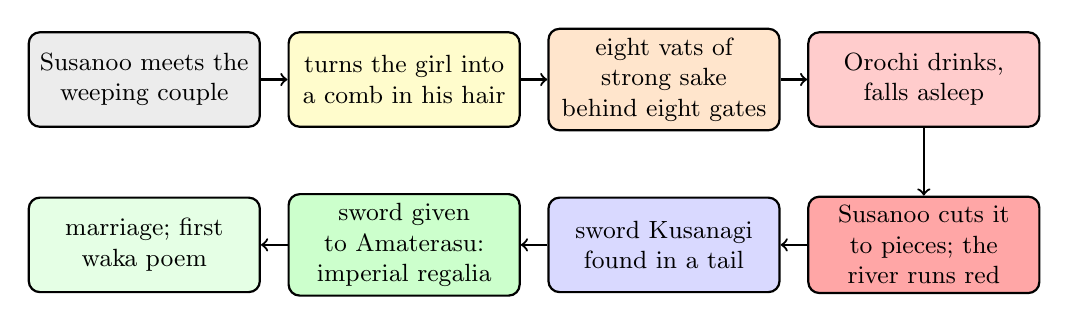
\begin{tikzpicture}[st/.style={draw, thick, rounded corners, align=center, font=\small, text width=2.7cm, minimum height=1.2cm}]
  \node[st, fill=gray!15] (1) at (0,0) {Susanoo meets the weeping couple};
  \node[st, fill=yellow!20] (2) at (3.3,0) {turns the girl into a comb in his hair};
  \node[st, fill=orange!20] (3) at (6.6,0) {eight vats of strong sake behind eight gates};
  \node[st, fill=red!20] (4) at (9.9,0) {Orochi drinks, falls asleep};
  \node[st, fill=red!35] (5) at (9.9,-2.1) {Susanoo cuts it to pieces; the river runs red};
  \node[st, fill=blue!15] (6) at (6.6,-2.1) {sword Kusanagi found in a tail};
  \node[st, fill=green!20] (7) at (3.3,-2.1) {sword given to Amaterasu: imperial regalia};
  \node[st, fill=green!10] (8) at (0,-2.1) {marriage; first waka poem};
  \draw[->, thick] (1) -- (2); \draw[->, thick] (2) -- (3); \draw[->, thick] (3) -- (4);
  \draw[->, thick] (4) -- (5); \draw[->, thick] (5) -- (6); \draw[->, thick] (6) -- (7);
  \draw[->, thick] (7) -- (8);
\end{tikzpicture}
\end{center}

\begin{itemize}
  \item The Orochi's body is as long as eight valleys and eight hills, with moss and trees
        growing on its back and a belly always bloody and inflamed.
  \item \textbf{Readings}: a personification of the flooding Hii river (its eight
        tributaries, red with iron sand); a memory of conquest of Izumo by Yamato; the
        iron-working culture of Izumo (the sword in the tail); a version of the
        widespread dragon-slayer / maiden-sacrifice tale (Perseus and Andromeda).
  \item \textbf{Kusanagi no Tsurugi} (\ja{草薙剣}, ``grass-cutting sword''): later used by
        the hero Yamato Takeru to escape a grass fire. One of the three regalia (mirror,
        sword, jewel).
\end{itemize}

\begin{aside}
Orochi has an enormous afterlife in popular culture: in \emph{Kagura} performances in
Shimane (with fireworks and long cloth-and-lantern serpents), in video games
(\emph{Ōkami}, \emph{Final Fantasy}, \emph{Warriors Orochi}), and as a model for
multi-headed kaijū such as King Ghidorah. The \emph{Kojiki} is the first ``monster
franchise''.
\end{aside}

\section{Other mythic creatures}

\begin{center}
\begin{tabular}{lp{10.5cm}}
\toprule
Creature & Story \\
\midrule
White hare of Inaba & tricks crocodiles (\emph{wani}, possibly sharks) into forming a bridge, is skinned, and is healed by the kind god Ōkuninushi \\
Yatagarasu \ja{八咫烏} & three-legged crow sent by heaven to guide Emperor Jinmu; now the emblem of the Japan Football Association \\
Wani \ja{和邇} & sea creatures; Toyotamahime, the sea king's daughter, gives birth in the form of a giant wani and leaves when her husband looks (another ``don't look'' story) \\
Earth spiders \ja{土蜘蛛} & \emph{tsuchigumo}, name for local people who resisted Yamato; later imagined as giant spider monsters (Noh, Raikō legends) \\
\bottomrule
\end{tabular}
\end{center}

\begin{remark}
The \emph{tsuchigumo} case is important: a term for human enemies of the state becomes,
over centuries, a literal monster. Monsters can be people who were ``monstered''
(Cohen's fourth thesis).
\end{remark}

\section*{Summary}
\begin{itemize}
  \item \emph{Kojiki} (712) and \emph{Nihon shoki} (720) are state-sponsored mythologies
        legitimating the imperial line.
  \item Izanagi and Izanami create the islands; Izanami's death and the flight from Yomi
        explain mortality and define death as pollution.
  \item Amaterasu, Tsukuyomi and Susanoo are born from Izanagi's purification.
  \item Susanoo kills the eight-headed Yamata no Orochi with sake and finds the sword
        Kusanagi.
  \item Mythic monsters can encode floods, conquest, iron-working and political enemies.
\end{itemize}
